% Source PDF page 481 (printed p. 467)
最小化 $\widetilde f$ 的步长。右端是简单二次函数，在 $t=1/M$ 时最小，最小值为 $f(x)-(1/(2M))\norm{\nabla f(x)}_2^2$。因此
\[
f(x^+)=\widetilde f(t_{\mathrm{exact}})
\le f(x)-\frac1{2M}\norm{\nabla f(x)}_2^2.
\]
两边减 $p^\star$，得到
\[
f(x^+)-p^\star\le f(x)-p^\star-\frac1{2M}\norm{\nabla f(x)}_2^2.
\]
结合（9.9）给出的 $\norm{\nabla f(x)}_2^2\ge2m(f(x)-p^\star)$，可得
\[
f(x^+)-p^\star\le(1-m/M)(f(x)-p^\star).
\]
递归应用，得到
\begin{equation}
f(x^{(k)})-p^\star\le c^k(f(x^{(0)})-p^\star),\tag{9.18}
\end{equation}
其中 $c=1-m/M<1$。因此 $k\to\infty$ 时 $f(x^{(k)})\to p^\star$。特别地，采用精确线搜索的梯度法，至多经过
\begin{equation}
\frac{\log((f(x^{(0)})-p^\star)/\epsilon)}{\log(1/c)}\tag{9.19}
\end{equation}
次迭代，就有 $f(x^{(k)})-p^\star\le\epsilon$。

虽然迭代次数的这一界较粗，但能帮助理解梯度法。分子
\[
\log((f(x^{(0)})-p^\star)/\epsilon)
\]
可解释为初始次优程度（$f(x^{(0)})$ 与 $p^\star$ 的间隙）与最终次优程度（小于 $\epsilon$）之比的对数。这提示迭代次数依赖初始点的好坏和最终所需精度。

界（9.19）的分母 $\log(1/c)$ 是 $M/m$ 的函数；已知 $M/m$ 是 $S$ 上 $\nabla^2f(x)$ 条件数的界，也是下水平集 $\{z\mid f(z)\le\alpha\}$ 条件数的界。当条件数界 $M/m$ 很大时，
\[
\log(1/c)=-\log(1-m/M)\approx m/M,
\]
所以迭代次数的界随 $M/m$ 增大而近似线性增长。

将会看到，若 $f$ 的Hessian在 $x^\star$ 附近条件数大，梯度法确实需要很多次迭代。反之，若 $f$ 的下水平集比较各向同性，使条件数界 $M/m$ 可取得较小，（9.18）说明收敛很快，因为 $c$ 小，至少不会太接近1。

（9.18）说明误差 $f(x^{(k)})-p^\star$ 至少像等比数列一样快地收敛于零。在迭代数值方法中，这称为\emph{线性收敛}，因为在误差对迭代次数的对数—线性图上，误差位于一条直线下方。

% Source PDF page 482 (printed p. 468)
\subsubsection*{回溯线搜索的分析}
再考虑梯度下降法采用回溯线搜索的情形。下面证明，凡 $0\le t\le1/M$，回溯退出条件
\[
\widetilde f(t)\le f(x)-\alpha t\norm{\nabla f(x)}_2^2
\]
都成立。首先注意
\[
0\le t\le1/M\ \Longrightarrow\ -t+\frac{Mt^2}{2}\le-t/2,
\]
这由 $-t+Mt^2/2$ 的凸性得到。结合界（9.17），对 $0\le t\le1/M$，
\[
\begin{aligned}
\widetilde f(t)&\le f(x)-t\norm{\nabla f(x)}_2^2
+\frac{Mt^2}{2}\norm{\nabla f(x)}_2^2\\
&\le f(x)-(t/2)\norm{\nabla f(x)}_2^2\\
&\le f(x)-\alpha t\norm{\nabla f(x)}_2^2,
\end{aligned}
\]
最后一步利用 $\alpha<1/2$。因此回溯线搜索终止时，或者 $t=1$，或者 $t\ge\beta/M$。由此得到目标减小量的下界。第一种情况下，
\[
f(x^+)\le f(x)-\alpha\norm{\nabla f(x)}_2^2;
\]
第二种情况下，
\[
f(x^+)\le f(x)-(\beta\alpha/M)\norm{\nabla f(x)}_2^2.
\]
综合起来，总有
\[
f(x^+)\le f(x)-\min\{\alpha,\beta\alpha/M\}\norm{\nabla f(x)}_2^2.
\]
接下来与精确线搜索完全一样。两边减 $p^\star$，得到
\[
f(x^+)-p^\star\le f(x)-p^\star
-\min\{\alpha,\beta\alpha/M\}\norm{\nabla f(x)}_2^2,
\]
结合 $\norm{\nabla f(x)}_2^2\ge2m(f(x)-p^\star)$，得到
\[
f(x^+)-p^\star
\le(1-\min\{2m\alpha,2\beta\alpha m/M\})(f(x)-p^\star).
\]
因此
\[
f(x^{(k)})-p^\star\le c^k(f(x^{(0)})-p^\star),
\]
其中
\[
c=1-\min\{2m\alpha,2\beta\alpha m/M\}<1.
\]
特别地，$f(x^{(k)})$ 至少与一个等比数列一样快地收敛于 $p^\star$，其指数至少部分取决于条件数界 $M/m$。用迭代方法术语说，收敛至少是线性的。

% Source PDF page 483 (printed p. 469)
\begin{figure}[htbp]\centering
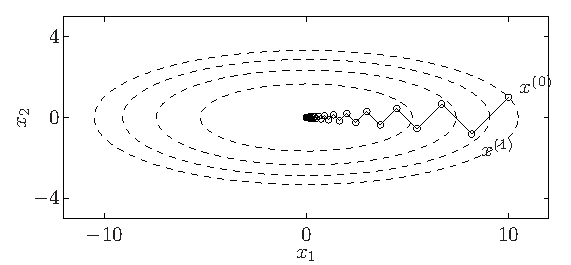
\includegraphics[width=.75\linewidth]{figures/ch09-fig02.pdf}
\caption*{图9.2\quad 函数 $f(x)=(1/2)(x_1^2+10x_2^2)$ 的若干等值线。其下水平集为椭球，条件数恰为10。图中显示从 $x^{(0)}=(10,1)$ 出发，采用精确线搜索的梯度法迭代点。}
\end{figure}
\subsection{例子}
\subsubsection*{$\R^2$ 中的二次问题}
第一个例子非常简单。考虑 $\R^2$ 上的二次目标函数
\[
f(x)=\tfrac12(x_1^2+\gamma x_2^2),
\]
其中 $\gamma>0$。显然，最优点为 $x^\star=0$，最优值为0。$f$ 的Hessian为常矩阵，特征值为1和 $\gamma$，因此所有下水平集的条件数都恰为
\[
\frac{\max\{1,\gamma\}}{\min\{1,\gamma\}}=\max\{\gamma,1/\gamma\}.
\]
强凸性常数 $m,M$ 最紧的选择为
\[
m=\min\{1,\gamma\},\qquad M=\max\{1,\gamma\}.
\]
从 $x^{(0)}=(\gamma,1)$ 出发，应用采用精确线搜索的梯度下降法。此时可求得迭代点 $x^{(k)}$ 及函数值的闭式表达式（习题9.6）：
\[
x_1^{(k)}=\gamma\left(\frac{\gamma-1}{\gamma+1}\right)^k,\qquad
x_2^{(k)}=\left(-\frac{\gamma-1}{\gamma+1}\right)^k,
\]
以及
\[
f(x^{(k)})=\frac{\gamma(\gamma+1)}2
\left(\frac{\gamma-1}{\gamma+1}\right)^{2k}
=\left(\frac{\gamma-1}{\gamma+1}\right)^{2k}f(x^{(0)}).
\]
图9.2显示 $\gamma=10$ 的情形。

这个简单例子的收敛恰为线性，即误差恰好构成等比数列，每次迭代乘以因子 $|(\gamma-1)/(\gamma+1)|^2$。

% Source PDF page 484 (printed p. 470)
$\gamma=1$ 时，一次迭代即得精确解；$\gamma$ 离1不远时（例如介于 $1/3$ 与3之间），收敛很快；$\gamma\gg1$ 或 $\gamma\ll1$ 时，收敛很慢。

可将收敛与§9.3.1所得界比较。取最不保守的 $m=\min\{1,\gamma\}$、$M=\max\{1,\gamma\}$，界（9.18）保证每次迭代误差至少缩小到原来的 $c=1-m/M$。实际上，误差每次恰好乘以
\[
\left(\frac{1-m/M}{1+m/M}\right)^2.
\]
对于对应大条件数的很小 $m/M$，上界（9.19）说明达到给定精度所需迭代次数至多按 $M/m$ 增长。本例中，实际次数近似按 $(M/m)/4$ 增长，即约为上界的四分之一。因此，对于这一简单例子，简单分析得到的迭代次数界只保守约四倍（采用最不保守的 $m,M$）。特别地，收敛速率及其上界都强烈依赖下水平集的条件数。

\subsubsection*{$\R^2$ 中的非二次问题}
再考虑 $\R^2$ 中非二次例子：
\begin{equation}
f(x_1,x_2)=e^{x_1+3x_2-0.1}
+e^{x_1-3x_2-0.1}+e^{-x_1-0.1}.\tag{9.20}
\end{equation}
采用回溯线搜索的梯度法，参数为 $\alpha=0.1,\beta=0.7$。图9.3显示 $f$ 的若干等值线和梯度法产生的迭代点 $x^{(k)}$（小圆圈）。连接相邻迭代点的线表示缩放后的步：
\[
x^{(k+1)}-x^{(k)}=-t^{(k)}\nabla f(x^{(k)}).
\]
图9.4显示误差 $f(x^{(k)})-p^\star$ 与迭代次数 $k$ 的关系。图表明误差近似按等比数列收敛于零，即近似线性收敛。本例中，误差在20次迭代内从约10降到约 $10^{-7}$，所以每次约乘 $10^{-8/20}\approx0.4$。我们的分析预见这种较快收敛，因为 $f$ 的下水平集条件不算太差，即 $M/m$ 可选得不太大。

为比较回溯与精确线搜索，在同一问题、同一初始点上使用精确线搜索的梯度法。结果见图9.5和9.4。收敛也近似线性，速率约为回溯线搜索梯度法的两倍。精确线搜索时，误差在15次迭代中约乘 $10^{-11}$，即每次约乘 $10^{-11/15}\approx0.2$。

% Source PDF page 485 (printed p. 471)
\begin{figure}[htbp]\centering
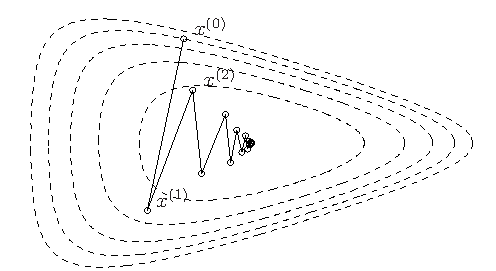
\includegraphics[width=.65\linewidth]{figures/ch09-fig03.pdf}
\caption*{图9.3\quad 采用回溯线搜索的梯度法的迭代点，目标为（9.20）的 $\R^2$ 问题。虚线为 $f$ 的等值线，小圆圈为迭代点。连接相邻迭代点的实线表示缩放后的步 $t^{(k)}\Delta x^{(k)}$。}
\end{figure}
\begin{figure}[htbp]\centering
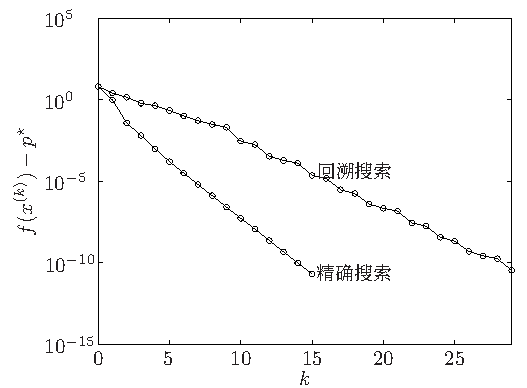
\includegraphics[width=.7\linewidth]{figures/ch09-fig04.pdf}
\caption*{图9.4\quad 对目标为（9.20）的 $\R^2$ 问题，回溯与精确线搜索梯度法的误差 $f(x^{(k)})-p^\star$ 随迭代次数 $k$ 的变化。图中近似线性收敛，回溯线搜索时误差每次迭代约乘0.4，精确线搜索时约乘0.2。}
\end{figure}

% Source PDF page 486 (printed p. 472)
\begin{figure}[htbp]\centering
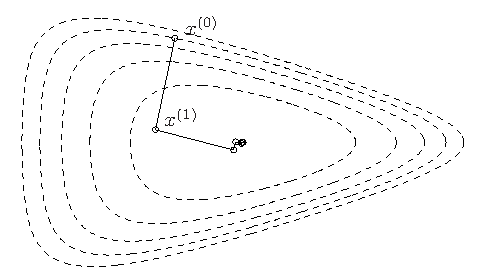
\includegraphics[width=.65\linewidth]{figures/ch09-fig05.pdf}
\caption*{图9.5\quad 对目标为（9.20）的 $\R^2$ 问题，采用精确线搜索的梯度法迭代点。}
\end{figure}
\subsubsection*{$\R^{100}$ 中的问题}
接着考虑较大例子，形式为
\begin{equation}
f(x)=c^\T x-\sum_{i=1}^m\log(b_i-a_i^\T x),\tag{9.21}
\end{equation}
有 $m=500$ 项、$n=100$ 个变量。

参数 $\alpha=0.1,\beta=0.5$ 的回溯线搜索梯度法的进展见图9.6。开始约20次迭代近似线性且较快收敛，随后转为较慢的线性收敛。总体而言，约175次迭代将误差缩小 $10^6$ 倍，平均每次误差约乘 $10^{-6/175}\approx0.92$。前20次的初始收敛率约为每次乘0.8；20次以后较慢的最终收敛率约为每次乘0.94。

图9.6还显示精确线搜索梯度法的收敛。仍近似线性，总体误差每次约乘 $10^{-6/140}\approx0.91$，只比回溯线搜索略快。

最后考察回溯参数 $\alpha,\beta$ 对收敛速率的影响，统计达到 $f(x^{(k)})-p^\star\le10^{-5}$ 所需迭代次数。第一个实验固定 $\beta=0.5$，将 $\alpha$ 从0.05变到0.5。所需次数从较大 $\alpha$（0.2--0.5）时的约80次，到较小 $\alpha$ 时的约170次。这些及其他实验表明，梯度法使用0.2--0.5间较大的 $\alpha$ 效果更好。

类似地，固定 $\alpha=0.1$，将 $\beta$ 从0.05变到0.95，可研究 $\beta$ 的影响。总次数变化同样不大，从 $\beta\approx0.5$ 时约80次，到 $\beta$ 很小或接近1时约200次。这些及其他实验表明，$\beta\approx0.5$ 是不错的选择。

% Source PDF page 487 (printed p. 473)
\begin{figure}[htbp]\centering
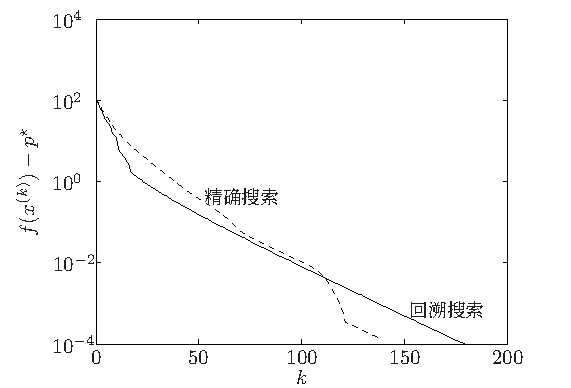
\includegraphics[width=.75\linewidth]{figures/ch09-fig06.pdf}
\caption*{图9.6\quad 对 $\R^{100}$ 中的一个问题，采用回溯和精确线搜索的梯度法误差 $f(x^{(k)})-p^\star$ 随迭代次数 $k$ 的变化。}
\end{figure}
这些实验表明，回溯参数对收敛的影响不大，约不超过两倍。

\subsubsection*{梯度法与条件数}
最后一个实验说明 $\nabla^2f(x)$（或下水平集）条件数对梯度法收敛速率的重要性。以（9.21）的函数开始，但用 $x=T\overline x$ 替换变量 $x$，其中
\[
T=\diag(1,\gamma^{1/n},\gamma^{2/n},\ldots,\gamma^{(n-1)/n}),
\]
即最小化
\begin{equation}
\overline f(\overline x)=c^\T T\overline x
-\sum_{i=1}^m\log(b_i-a_i^\T T\overline x).\tag{9.22}
\end{equation}
这给出以 $\gamma$ 为参数的一族优化问题，$\gamma$ 影响问题条件数。

图9.7显示采用 $\alpha=0.3,\beta=0.7$ 的回溯线搜索时，达到
$\overline f(\overline x^{(k)})-\overline p^\star<10^{-5}$ 所需次数关于 $\gamma$ 的函数。即使对角缩放仅为10:1（$\gamma=10$），次数也超过一千；对角缩放达到20或更大时，梯度法就慢到基本无法使用。

图9.8显示最优点处Hessian $\nabla^2\overline f(\overline x^\star)$ 的条件数。$\gamma$ 很大或很小时，条件数约按 $\max\{\gamma^2,1/\gamma^2\}$ 增长，与迭代次数关于 $\gamma$ 的关系非常相似。这再次说明，条件与收敛速度之间的关系是实际现象，而非分析造成的假象。

% Source PDF page 488 (printed p. 474)
\begin{figure}[htbp]\centering
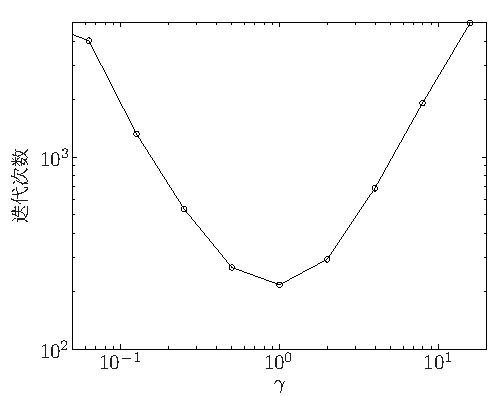
\includegraphics[width=.65\linewidth]{figures/ch09-fig07.pdf}
\caption*{图9.7\quad 梯度法用于（9.22）时的迭代次数。纵轴为达到 $\overline f(\overline x^{(k)})-\overline p^\star<10^{-5}$ 所需次数，横轴为控制对角缩放程度的参数 $\gamma$。采用 $\alpha=0.3,\beta=0.7$ 的回溯线搜索。}
\end{figure}
\begin{figure}[htbp]\centering
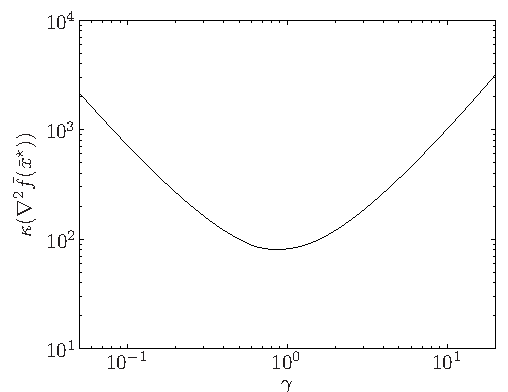
\includegraphics[width=.65\linewidth]{figures/ch09-fig08.pdf}
\caption*{图9.8\quad 函数最小点处Hessian条件数关于 $\gamma$ 的函数。与图9.7比较可见，条件数对收敛速率有很强的影响。}
\end{figure}

% Source PDF page 489 (printed p. 475)
\subsubsection*{结论}
根据上述及其他数值例子，可归纳以下结论。
\begin{itemize}
\item 梯度法常表现出近似线性收敛，即误差 $f(x^{(k)})-p^\star$ 近似按等比数列收敛于零。
\item 回溯参数 $\alpha,\beta$ 的选择对收敛有可察觉但不剧烈的影响。精确线搜索有时改善梯度法收敛，但影响不大（可能不值得为此专门实现精确线搜索）。
\item 收敛速率强烈依赖Hessian或下水平集的条件数。即使问题条件尚可（如条件数为几百），收敛也可能很慢。条件数更大（如1000或以上）时，梯度法慢到实践中无法使用。
\end{itemize}
梯度法的主要优点是简单，主要缺点则是收敛速率对Hessian或下水平集条件数过于敏感。

\section{最速下降法}
$f(x+v)$ 在 $x$ 附近的一阶Taylor近似为
\[
f(x+v)\approx\widehat f(x+v)=f(x)+\nabla f(x)^\T v.
\]
右端第二项 $\nabla f(x)^\T v$ 是 $f$ 在 $x$ 处沿 $v$ 的方向导数，给出小步 $v$ 引起的函数近似变化。若方向导数为负，$v$ 就是下降方向。

现讨论如何选择 $v$，使方向导数尽可能负。由于 $\nabla f(x)^\T v$ 关于 $v$ 线性，只要 $v$ 是下降方向，即 $\nabla f(x)^\T v<0$，就可以将 $v$ 放大，使方向导数任意负。为使问题合理，必须限制 $v$ 的大小，或用其长度归一化。

设 $\norm{\cdot}$ 为 $\R^n$ 的任意范数。定义相对于此范数的\emph{归一化最速下降方向}为
\begin{equation}
\Delta x_{\mathrm{nsd}}=
\argmin\{\nabla f(x)^\T v\mid\norm v=1\}.\tag{9.23}
\end{equation}
（称“一个”最速下降方向，因为可能有多个最小点。）归一化最速下降方向 $\Delta x_{\mathrm{nsd}}$ 是单位范数的步，使 $f$ 的线性近似下降最多。

其几何解释如下。也可将 $\Delta x_{\mathrm{nsd}}$ 定义为
\[
\Delta x_{\mathrm{nsd}}=
\argmin\{\nabla f(x)^\T v\mid\norm v\le1\},
\]

% Source PDF page 490 (printed p. 476)
即范数 $\norm{\cdot}$ 的单位球内，沿 $-\nabla f(x)$ 方向延伸最远的方向。

将归一化方向按特定方式缩放，考虑未归一化的\emph{最速下降步} $\Delta x_{\mathrm{sd}}$ 也很方便：
\begin{equation}
\Delta x_{\mathrm{sd}}=\norm{\nabla f(x)}_*\Delta x_{\mathrm{nsd}},\tag{9.24}
\end{equation}
其中 $\norm{\cdot}_*$ 表示对偶范数。注意，最速下降步满足
\[
\nabla f(x)^\T\Delta x_{\mathrm{sd}}
=\norm{\nabla f(x)}_*\nabla f(x)^\T\Delta x_{\mathrm{nsd}}
=-\norm{\nabla f(x)}_*^2
\]
（见习题9.7）。最速下降法以最速下降方向为搜索方向。

\begin{origalgorithm}{9.4}
\emph{最速下降法。}

给定初始点 $x\in\dom f$。

重复：
\begin{enumerate}
\item 计算最速下降方向 $\Delta x_{\mathrm{sd}}$。
\item \emph{线搜索。}通过回溯或精确线搜索选择 $t$。
\item \emph{更新。}$x:=x+t\Delta x_{\mathrm{sd}}$。
\end{enumerate}
直到满足停止准则。
\end{origalgorithm}

使用精确线搜索时，方向中的缩放因子不影响结果，因此可使用归一化或未归一化方向。

\subsection{欧几里得范数和二次范数下的最速下降}
\subsubsection*{欧几里得范数下的最速下降}
若 $\norm{\cdot}$ 取欧几里得范数，最速下降方向就是负梯度，即 $\Delta x_{\mathrm{sd}}=-\nabla f(x)$。欧几里得范数下的最速下降法与梯度下降法一致。

\subsubsection*{二次范数下的最速下降}
考虑二次范数
\[
\norm z_P=(z^\T Pz)^{1/2}=\norm{P^{1/2}z}_2,
\]
其中 $P\in\mathbf S_{++}^n$。归一化最速下降方向为
\[
\Delta x_{\mathrm{nsd}}
=-\bigl(\nabla f(x)^\T P^{-1}\nabla f(x)\bigr)^{-1/2}P^{-1}\nabla f(x).
\]
对偶范数为 $\norm z_*=\norm{P^{-1/2}z}_2$，所以相对于 $\norm{\cdot}_P$ 的最速下降步为
\begin{equation}
\Delta x_{\mathrm{sd}}=-P^{-1}\nabla f(x).\tag{9.25}
\end{equation}
图9.9说明二次范数的归一化最速下降方向。
